\documentclass[12pt]{article}%
\usepackage{amsfonts}
\usepackage{fancyhdr}
\usepackage{comment}
\usepackage[a4paper, top=2.5cm, bottom=2.5cm, left=2.2cm, right=2.2cm]%
{geometry}
\usepackage{times}
\usepackage{amsmath}
\usepackage{changepage}
\usepackage{amssymb}
\usepackage{graphicx}%
\setcounter{MaxMatrixCols}{30}
%\usepackage{hyperref}


%These tell TeX which packages to use.
\usepackage{array,epsfig}
\usepackage{amsmath}
\usepackage{amsfonts}
\usepackage{amssymb}
\usepackage{amsxtra}
\usepackage{amsthm}
\usepackage{mathrsfs}
\usepackage{color}





\usepackage{listings}
\usepackage{longtable}
\definecolor{codegreen}{rgb}{0,0.6,0}
\definecolor{codegray}{rgb}{0.5,0.5,0.5}
\definecolor{codepurple}{rgb}{0.58,0,0.82}
\definecolor{backcolour}{rgb}{0.96,0.96,0.94}
\lstdefinestyle{mystyle}{
	backgroundcolor=\color{backcolour},
	commentstyle=\color{codegreen},
	keywordstyle=\color{blue},
	numberstyle=\tiny\color{codegray},
	stringstyle=\color{codepurple},
	basicstyle=\footnotesize,
	breakatwhitespace=false,
	breaklines=true,
	captionpos=b,
	keepspaces=true,
	numbers=left,
	numbersep=5pt,
	showspaces=false,
	showstringspaces=false,
	showtabs=false,
	tabsize=2
}
\lstset{style=mystyle}

















%%%%%%%%% hyperref %%%%%%%%%%%%
\usepackage[pdftex,letterpaper=true,pdfpagelabels=true,pagebackref=true,bookmarks]{hyperref} 
% with basic options
% pagebackref=true provides links back from the References to the body text. This can cause trouble for printing.

%%%%%%%% cref cleverref %%%%%%%%%%%

% cref package must be loaded after hyperref !
\usepackage[noabbrev]{cleveref}




%Here I define some theorem styles and shortcut commands for symbols I use often
\theoremstyle{definition}
\newtheorem{defn}{Definition}
\newtheorem{thm}{Theorem}
\newtheorem*{thm*}{Theorem}
\newtheorem{cor}{Corollary}
\newtheorem*{rmk}{Remark}
\newtheorem{lem}{Lemma}
\newtheorem*{joke}{Joke}
\newtheorem{ex}{Example}
\newtheorem*{soln}{Solution}
\newtheorem{prop}{Proposition}




\newtheorem{sol}{Solution}


\newtheorem{theorem}{Theorem}
\newtheorem{acknowledgement}[theorem]{Acknowledgement}
\newtheorem{algorithm}[theorem]{Algorithm}
\newtheorem{axiom}{Axiom}
\newtheorem{case}[theorem]{Case}
\newtheorem{claim}[theorem]{Claim}
\newtheorem{conclusion}[theorem]{Conclusion}
\newtheorem{condition}[theorem]{Condition}
\newtheorem{conjecture}[theorem]{Conjecture}
\newtheorem{corollary}[theorem]{Corollary}
\newtheorem{criterion}[theorem]{Criterion}
\newtheorem{definition}[theorem]{Definition}
\newtheorem{example}[theorem]{Example}
\newtheorem{exercise}[theorem]{Exercise}
\newtheorem{lemma}[theorem]{Lemma}
\newtheorem{notation}[theorem]{Notation}
\newtheorem{problem}[theorem]{Problem}
\newtheorem{proposition}[theorem]{Proposition}
\newtheorem{remark}[theorem]{Remark}
\newtheorem{solution}[theorem]{Solution}
\newtheorem{summary}[theorem]{Summary}
%\newenvironment{proof}[1][Proof]{\textbf{#1.} }{\ \rule{0.5em}{0.5em}}

\newcommand{\Q}{\mathbb{Q}}
\newcommand{\R}{\mathbb{R}}
\newcommand{\C}{\mathbb{C}}
\newcommand{\Z}{\mathbb{Z}}


% operators
\DeclareMathOperator{\rank}{{rank}}
\DeclareMathOperator{\argmin}{{argmin}}
\DeclareMathOperator{\argmax}{{argmax}}
\DeclareMathOperator{\flatt}{{flat}}
\DeclareMathOperator{\sym}{{sym}}
\DeclareMathOperator{\sgn}{sgn}
\DeclareMathOperator{\conv}{conv}
\DeclareMathOperator{\env}{env}
\DeclareMathOperator{\dist}{dist}
\DeclareMathOperator{\epi}{epi}
\DeclareMathOperator{\Id}{Id}
\DeclareMathOperator{\dom}{dom}
\DeclareMathOperator{\cl}{cl}
\DeclareMathOperator{\Normal}{Normal}


% matrices
\newcommand{\bbm}{\begin{bmatrix}}
\newcommand{\ebm}{\end{bmatrix}}
\newcommand{\bem}{\begin{pmatrix}}
\newcommand{\eem}{\end{pmatrix}}

% parentheses
%\newcommand{\l[}{\left[}
%\newcommand{\r]}{\right]}
%\newcommand{\l(}{\left(}
%\newcommand{\r)}{\right)}

% 
\def\<{\langle}
\def\>{\rangle}

\usepackage{cite}



%%%%%%%%%%%% Mathcal{ } %%%%%%%
%%%%%%%%%%%%%%%%%%%%%%%%%%%%%%%
\newcommand{\cA}{{\mathcal A}}
\newcommand{\cB}{{\mathcal B}}
\newcommand{\cC}{{\mathcal C}}
\newcommand{\cD}{{\mathcal D}}
\newcommand{\cE}{{\mathcal E}}
\newcommand{\cF}{{\mathcal F}}
\newcommand{\cG}{{\mathcal G}}
\newcommand{\cDQ}{{\mathcal {DQ}}}
\newcommand{\cH}{{\mathcal H}}
\newcommand{\cI}{{\mathcal I}}
\newcommand{\cJ}{{\mathcal J}}
\newcommand{\cK}{{\mathcal K}}
\newcommand{\cL}{{\mathcal L}}
\newcommand{\cM}{{\mathcal M}}
\newcommand{\cN}{{\mathcal N}}
\newcommand{\cO}{{\mathcal O}}
\newcommand{\cP}{{\mathcal P}}
\newcommand{\cQ}{{\mathcal Q}}
\newcommand{\cR}{{\mathcal R}}
\newcommand{\cS}{{\mathcal S}}
\newcommand{\cT}{{\mathcal T}}
\newcommand{\cDP}{{\mathcal {DP}}}
\newcommand{\cU}{{\mathcal U}}
\newcommand{\cV}{{\mathcal V}}
\newcommand{\cW}{{\mathcal W}}
\newcommand{\cX}{{\mathcal X}}
\newcommand{\cY}{{\mathcal Y}}
\newcommand{\cZ}{{\mathcal Z}}

%%%%%%%%%%%% Mathbb{ } %%%%%%%%
%%%%%%%%%%%%%%%%%%%%%%%%%%%%%%%
\newcommand{\bA}{{\mathbb A}}
\newcommand{\bB}{{\mathbb B}}
\newcommand{\bC}{{\mathbb C}}
\newcommand{\bD}{{\mathbb D}}
\newcommand{\bE}{{\mathbb E}}
\newcommand{\bF}{{\mathbb F}}
\newcommand{\bG}{{\mathbb G}}
\newcommand{\bH}{{\mathbb H}}
\newcommand{\bI}{{\mathbb I}}
\newcommand{\bJ}{{\mathbb J}}
\newcommand{\bK}{{\mathbb K}}
\newcommand{\bL}{{\mathbb L}}
\newcommand{\bM}{{\mathbb M}}
\newcommand{\bN}{{\mathbb N}}
\newcommand{\bO}{{\mathbb O}}
\newcommand{\bP}{{\mathbb P}}
\newcommand{\bQ}{{\mathbb Q}}
\newcommand{\bR}{{\mathbb R}}
\newcommand{\bS}{{\mathbb S}}
\newcommand{\bT}{{\mathbb T}}
\newcommand{\bU}{{\mathbb U}}
\newcommand{\bV}{{\mathbb V}}
\newcommand{\bW}{{\mathbb W}}
\newcommand{\bX}{{\mathbb X}}
\newcommand{\bY}{{\mathbb Y}}
\newcommand{\bZ}{{\mathbb Z}}



\begin{document}
	
	\title{CPSC 532W Homework 3}
	\author{Naomi Graham}
	\date{\today}
	\maketitle
	
	All the code can be found on: \url{https://github.com/n6graham/cpsc532_hw3}.
	
	
	
	\section{Importance sampling}
	
	\subsection{Code}
	For Importance Sampling I used the evaluation-based implementation based off of Jason's HW2 code.
	
	
	\begin{lstlisting}[language=Python ]
	def evaluate_program(ast):
	    """Evaluate a program as desugared by daphne, generate a sample from the prior
	    Args:
	        ast: json FOPPL program
	    Returns: sample from the prior of ast
	    """
	    PROCS = {} #program procedures
	    for i in range(len(ast)-1):
	        proc = ast[i]
	        proc_name, proc_arg_names, proc_expr = proc[1], proc[2], proc[3]
	        PROCS[proc_name] = (proc_arg_names,proc_expr)
	
	    #print(PROCS)
	    # expr is ast[-1]
	
	
	    def eval(expr, sigma, scope):
	        if is_const(expr, scope):
	            if type(expr) in [int, float]:
	                expr = torch.Tensor([expr]).squeeze()
	            return expr, sigma
	        elif is_var(expr, scope):
	            return scope[expr], sigma
	        elif is_let(expr, scope):
	            var_name, sub_expr, final_expr = expr[1][0], expr[1][1], expr[2]
	            var_value, sigma = eval(sub_expr, sigma, scope)
	            return eval(final_expr, sigma, {**scope, var_name: var_value})
	        elif is_if(expr,scope):
	            cond_expr, true_expr, false_expr = expr[1], expr[2], expr[3]
	            cond_value, sigma = eval(cond_expr, sigma, scope)
	            if cond_value:
	                return eval(true_expr, sigma, scope)
	            else:
	                return eval(false_expr, sigma, scope)
	        elif is_sample(expr,scope):
	            dist_expr = expr[1]
	            dist_obj, sigma = eval(dist_expr,sigma,scope)
	            return dist_obj.sample(), sigma
	        elif is_observe(expr,scope):
	            # need to do something special here
	            dist_expr, obs_expr = expr[1], expr[2]
	            dist_obj, sigma = eval(dist_expr,sigma,scope)
	            obs_value, sigma = eval(obs_expr,sigma,scope)
	            sigma['logW'] = sigma['logW'] + dist_obj.log_prob(obs_value)
	            return obs_value, sigma
	        else:
	            proc_name = expr[0]
	            consts = []
	            for i in range(1,len(expr)):
	                const, sigma = eval(expr[i],sigma,scope)
	                consts.append(const)
	            if proc_name in PROCS:
	                proc_arg_names, proc_expr = PROCS[proc_name]
	                new_scope = {**scope}
	                for i, name in enumerate(proc_arg_names):
	                    new_scope[name] = consts[i]
	                return eval(proc_expr, sigma, new_scope)
	            else:
	                return PRIMITIVES[proc_name](*consts), sigma
	
	
	    return eval(ast[-1],{'logW':0}, {})
	\end{lstlisting}
	
	I also defined some extra functions: likelihood-weighting, compute-expectation, and compute-variance.
	
	\begin{lstlisting}[language=Python]
	def likelihood_weighting(L,ast):
	    weighted_samples = []
	
	    for i in range(0,L):
	        r, sigma = evaluate_program(ast)
	        #r, sigma = eval(e, {'logW':0}, [])
	        logW = sigma['logW']
	        weighted_samples.append((r,logW))
	        
	    return weighted_samples
	\end{lstlisting}
	
	\begin{lstlisting}[language=Python]
	def compute_expectation(weighted_samples):
	    '''
	    using a stream of weighted samples, compute according
	    to eq 4.6 
	    '''
	    L = len(weighted_samples)
	    log_weights = [weighted_samples[i][1] for i in range(0,L)]
	    weights = np.exp(np.array(log_weights))
	    print(weights)
	    r = [ weighted_samples[i][0] for i in range(0,L)]
	    denom = sum(weights)
	    print("denominator is", denom)
	    numerator = sum( [r[i] * weights[i] for i in range(0,L) ])
	    #numerator = sum( [weighted_samples[i][0] * weighted_samples[i][1] for i in range(0,L) ])
	
	    return numerator/denom
	\end{lstlisting}
		
	\begin{lstlisting}[language=Python]
	def compute_variance(weighted_samples, mu):
	
	    L = len(weighted_samples)
	    log_weights = [weighted_samples[i][1] for i in range(0,L)]
	    weights = np.exp(np.array(log_weights))
	    r = [ weighted_samples[i][0] for i in range(0,L)]
	    denom = sum(weights)
	    numerator = sum( [ (torch.square(r[i]) - torch.square(mu)) * weights[i] for i in range(0,L) ])
	    return numerator/denom
	\end{lstlisting}
	
	\subsection{results}
	
	The values returned are:
	
	Program 1:
	
	expectation is: tensor(7.2086)
	variance is tensor(0.7626) 
	 
	
	Program 2
	 
	expectation is: tensor([ 2.1571, -0.5566])
	variance is tensor([0.0561, 0.8358]) 
	 
	
	Program 3:
	 
	expectation is: tensor(0.7429)
	variance is tensor(0.1910) 
	 
	
	Program 4: 
	 
	expectation is: tensor(0.3221)
	variance is tensor(0.2183) 
	
	
	
	
	
	\section{MH within Gibbs}
	
	\subsection{code}
	For MH withing Gibbs I used a graph-based implementation based off of Jason's HW2 code.
	
	\begin{lstlisting}[language=Python]
def deterministic_eval(exp):
    "Evaluation function for the deterministic target language of the graph based representation."
    if type(exp) is list:
        op = exp[0]
        args = exp[1:]
        return env[op](*map(deterministic_eval, args))
    elif type(exp) in [int, float]:
        # We use torch for all numerical objects in our evaluator
        return torch.Tensor([float(exp)]).squeeze()
    elif type(exp) is torch.Tensor:
        return exp
    elif type(exp) is bool:
        return torch.tensor(exp)
    else:
        print("expression is:", exp)
        print(type(exp))
        raise Exception("Expression type unknown.", exp)

def topological_sort(nodes, edges):
    result = []
    visited = {}
    def helper(node):
        if node not in visited:
            visited[node] = True
            if node in edges:
                for child in edges[node]:
                    helper(child)
            result.append(node)
    for node in nodes:
        helper(node)
    return result[::-1]

def plugin_parent_values(expr, trace):
    if type(expr) == str and expr in trace:
        return trace[expr]
    elif type(expr) == list:
        return [plugin_parent_values(child_expr, trace) for child_expr in expr]
    else:
        return expr

def sample_from_joint(graph):
    "This function does ancestral sampling starting from the prior."
    # TODO insert your code here
    """
    1. Run topological sort on V using V and A, resulting in an array of v's
    2. Iterate through sample sites of the sorted array, and save sampled results on trace dictionary using P and Y
    - If keyword is sample*, first recursively replace sample site names with trace values in the expression from P. Then, run deterministic_eval.
    - If keyword is observe*, put the observation value in the trace dictionary
    3. Filter the trace dictionary for things sample sites you should return
    """
    procs, model, expr = graph[0], graph[1], graph[2]
    nodes, edges, links, obs = model['V'], model['A'], model['P'], model['Y']
    sorted_nodes = topological_sort(nodes, edges)

    sigma = {}
    trace = {}
    for node in sorted_nodes:
        keyword = links[node][0]
        if keyword == "sample*":
            link_expr = links[node][1]
            link_expr = plugin_parent_values(link_expr, trace)
            dist_obj  = deterministic_eval(link_expr)
            trace[node] = dist_obj.sample()
        elif keyword == "observe*":
            trace[node] = obs[node]

    expr = plugin_parent_values(expr, trace)
    return deterministic_eval(expr), sigma, trace
	\end{lstlisting}
	
	
	I added the function MH-Gibbs which also contains functions accept and Gibbs-step.
	\begin{lstlisting}[language=Python]
	def MH_Gibbs(graph, numsamples):
	    model = graph[1]
	    vertices = model['V']
	    arcs = model['A']
	    links = model['P'] # link functions aka P
	
	    # sort vertices for ancestral sampling
	    V_sorted = topological_sort(vertices,arcs)
	
	    def accept(x, cX, cXnew, Q):
	        # compute acceptance ratio to decide whether
	        # we keep cX or accept a new sample/trace cXnew
	        # cX and cXnew are the proposal mappings (dictionaries)
	        # which assign values to latent variables
	
	        # cXnew corresponds to the values for the new samples
	
	        # take the proposal distribution for the current vertex
	        # this is Q(x)
	        Qx = Q[x][1]
	
	        # we will sample from this with respect to cX and cXnew
	
	        # the difference comes from how we evaluate parents 
	        # plugging into eval
	        p = plugin_parent_values(Qx,cX)
	        pnew = plugin_parent_values(Qx,cXnew)
	
	        # p = Q(x)[X := \mathcal X]
	        # p' = Q(x)[X := \mathcal X']
	        # note that in this case we only need to worry about
	        # the parents of x to sample from the proposal
	
	
	        # evaluate 
	        d = deterministic_eval(p) # d = EVAL(p)
	        dnew = deterministic_eval(pnew) #d' = EVAL(p')
	
	        ### compute acceptance ratio ###
	
	        # initialize log alpha
	        logAlpha = dnew.log_prob(cXnew[x]) - d.log_prob(cX[x])
	
	        ### V_x = {x} \cup {v:x \in PA(v)} ###
	        startindex = V_sorted.index(x)
	        Vx = V_sorted[startindex:]
	
	        # compute alpha
	        for v in Vx:
	            Pv = links[v] # getting a bug here
	            v_exp = plugin_parent_values(Pv,cX) #same as we did for p and pnew
	            v_exp_new = plugin_parent_values(Pv,cXnew)
	            dv_new = deterministic_eval(v_exp_new[1])
	            dv = deterministic_eval(v_exp[1])
	
	            
	            ## change below
	            logAlpha = logAlpha + dv_new.log_prob(cXnew[v])
	            logAlpha = logAlpha - dv.log_prob(cX[v])
	        return torch.exp(logAlpha)
	
	    
	    def Gibbs_step(cX,Q):
	        # here we need a list of the latent (unobserved) variables
	        Xobsv = list(filter(lambda v: links[v][0] == "sample*", V_sorted))
	
	        for u in Xobsv:
	            # here we are doing the step
	            # d <- EVAL(Q(u) [X := \cX]) 
	            # note it suffices to consider only the non-observed variables
	            Qu = Q[u][1]
	            u_exp = plugin_parent_values(Qu,cX)
	            dist_u = deterministic_eval(u_exp).sample()
	            cXnew = {**cX}
	            cX[u] = dist_u
	
	            #compute acceptance ratio
	            alpha = accept(u,cX,cXnew,Q)
	            val = Uniform(0,1).sample()
	
	            if val < alpha:
	                cX = cXnew
	        return cX
	
	
	    Q = links # initialize the proposal with P (i.e. using the prior)
	    cX_list = [ sample_from_joint(graph)[2] ] # initialize the state/trace
	
	    for i in range(1,numsamples):
	        cX_0 = {**cX_list[i-1]} #make a copy of the trace
	        cX = Gibbs_step(cX_0,Q)
	        cX_list.append(cX)
	    
	    samples = list(map(lambda cX: deterministic_eval(plugin_parent_values(graph[2], cX)), cX_list))
	    #samples = [ deterministic_eval(plugin_parent_values(graph[2],X)) for X in cX_list ]
	
	    return samples
	\end{lstlisting}
		
	\newpage
	
	
	\subsection{Results}
	
	Here are the results from running MH Gibbs for programs 1 through 4:
	\begin{figure}[h]
	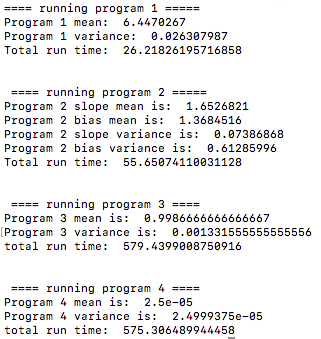
\includegraphics[scale=0.7]{MH_Gibbs_results}
	\end{figure}
	
	\newpage
	
	\subsubsection{Program 1}
	
	\begin{figure}[h]
	\centering
	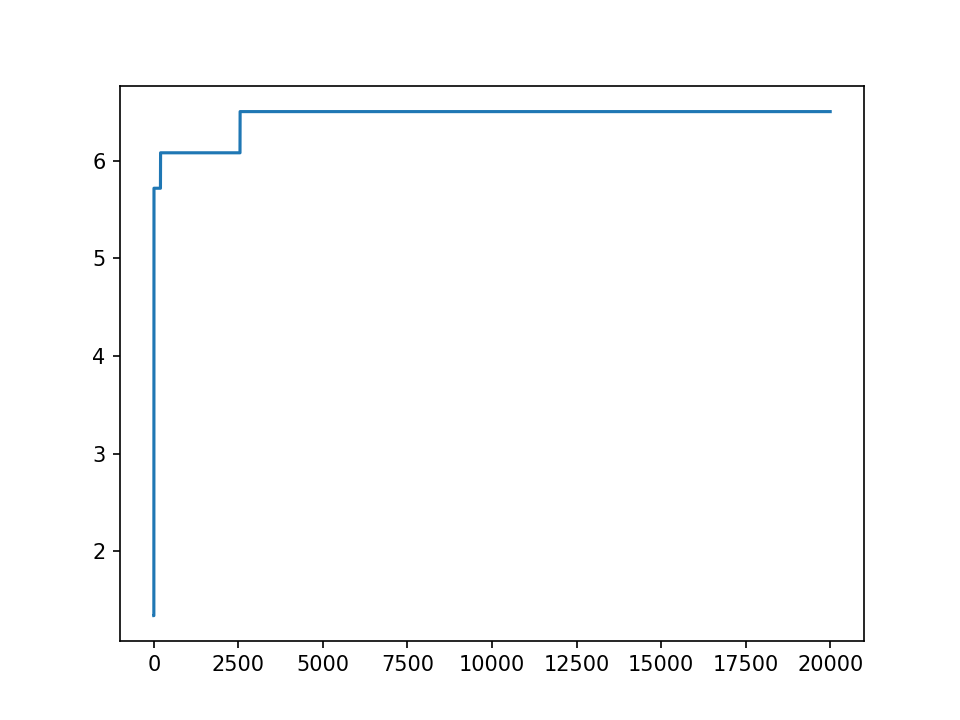
\includegraphics[scale=0.4]{p1traceplot.png}
	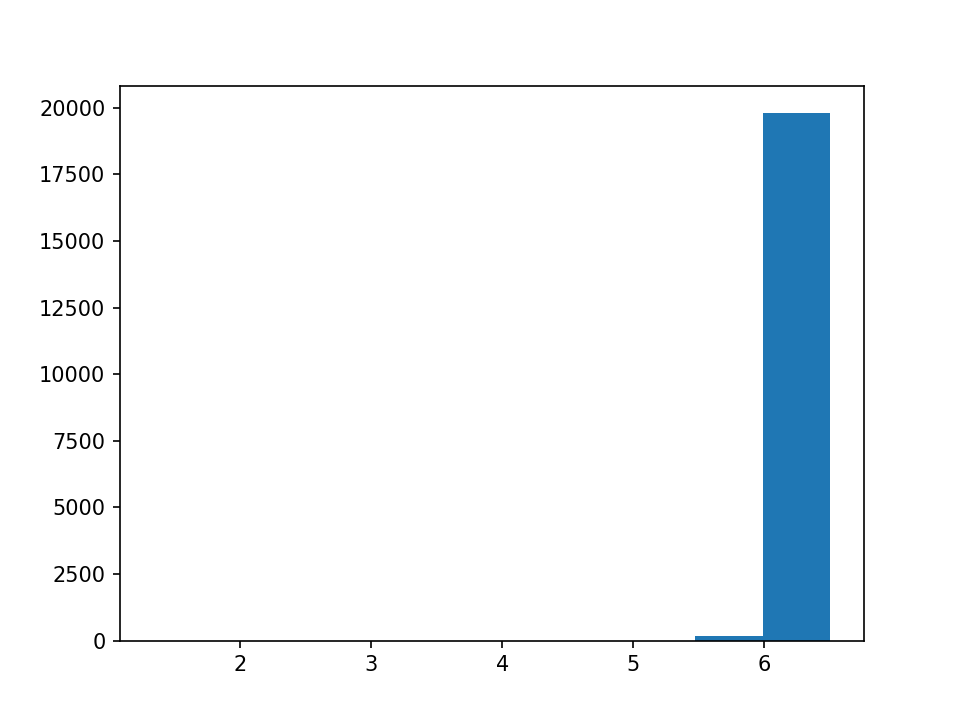
\includegraphics[scale=0.4]{p1histogram.png}
	\caption{trace plot (left) and histogram (right)}
	\end{figure}


	\subsubsection{Program 2}
	
	\begin{figure}[h]
	\centering
	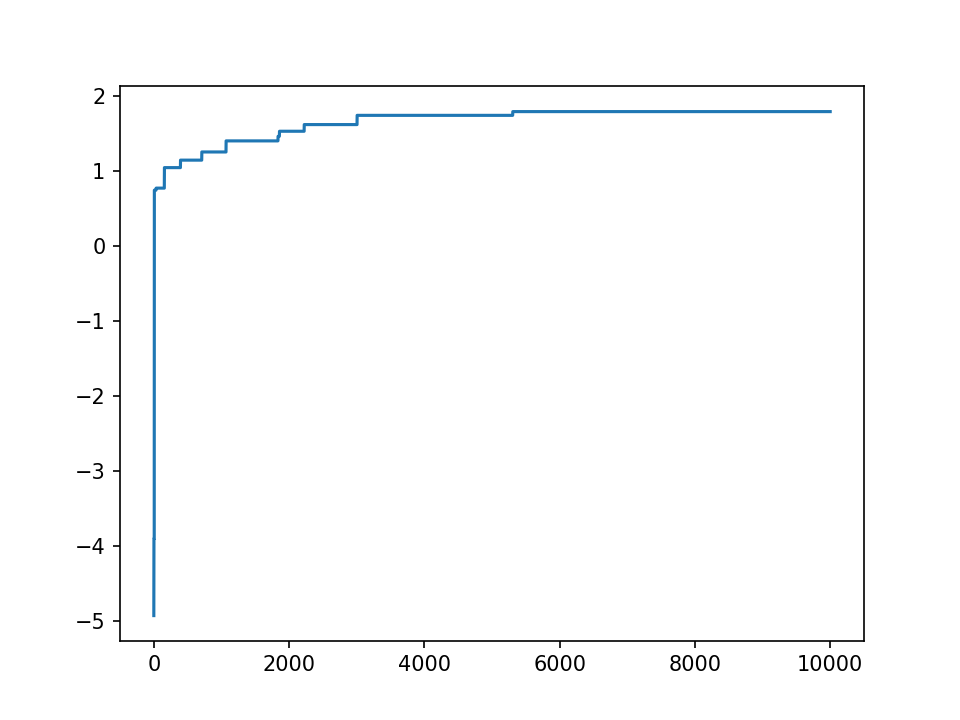
\includegraphics[scale=0.4]{p2traceplot_bias.png}
	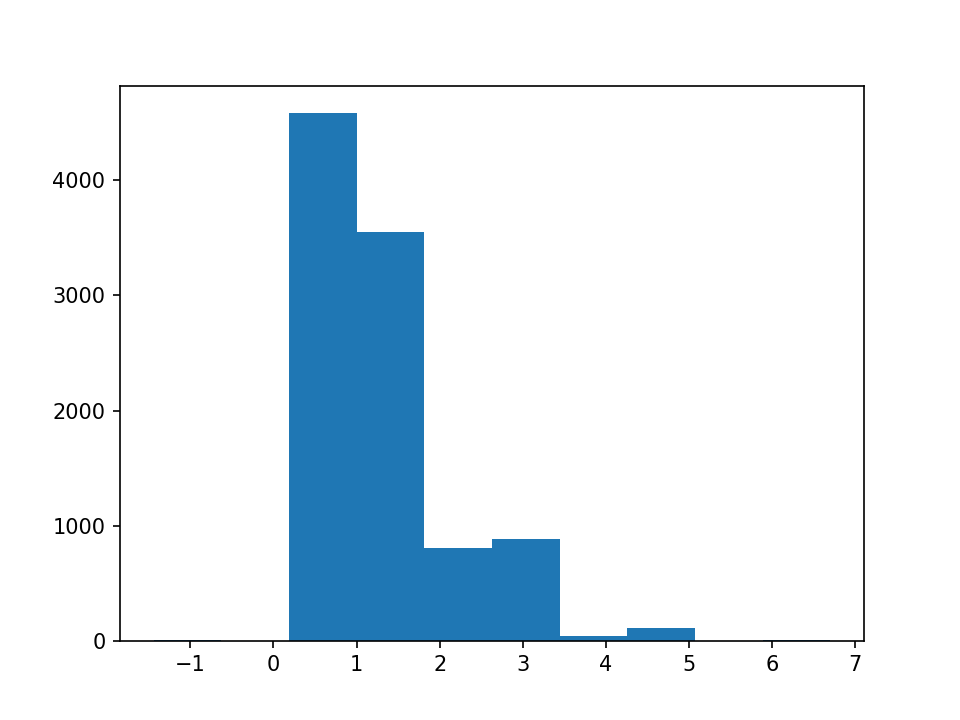
\includegraphics[scale=0.4]{p2histogram_bias.png}
	\caption{Program 2 (bias): trace plot (left) and histogram (right)}
	\end{figure}
	
	\begin{figure}[h]
	\centering
	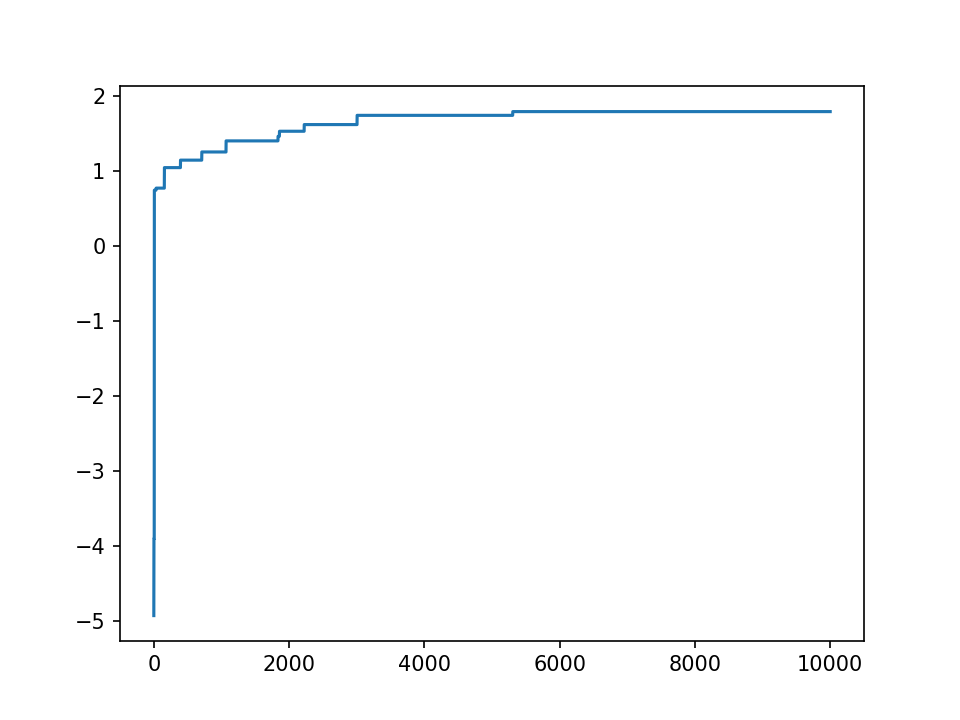
\includegraphics[scale=0.4]{p2traceplot_slope.png}
	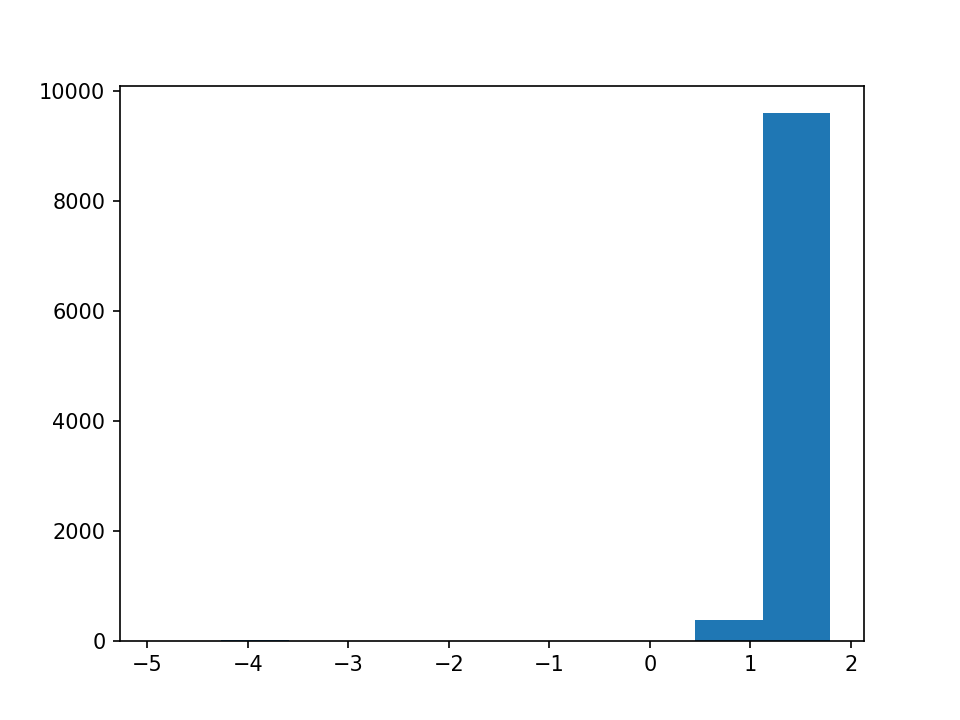
\includegraphics[scale=0.4]{p2histogram_slope.png}
	\caption{Program 2 (slope): trace plot (left) and histogram (right)}
	\end{figure}
		
	
		
	\subsubsection{Program 3}
	
	\begin{figure}[h]
		\centering
		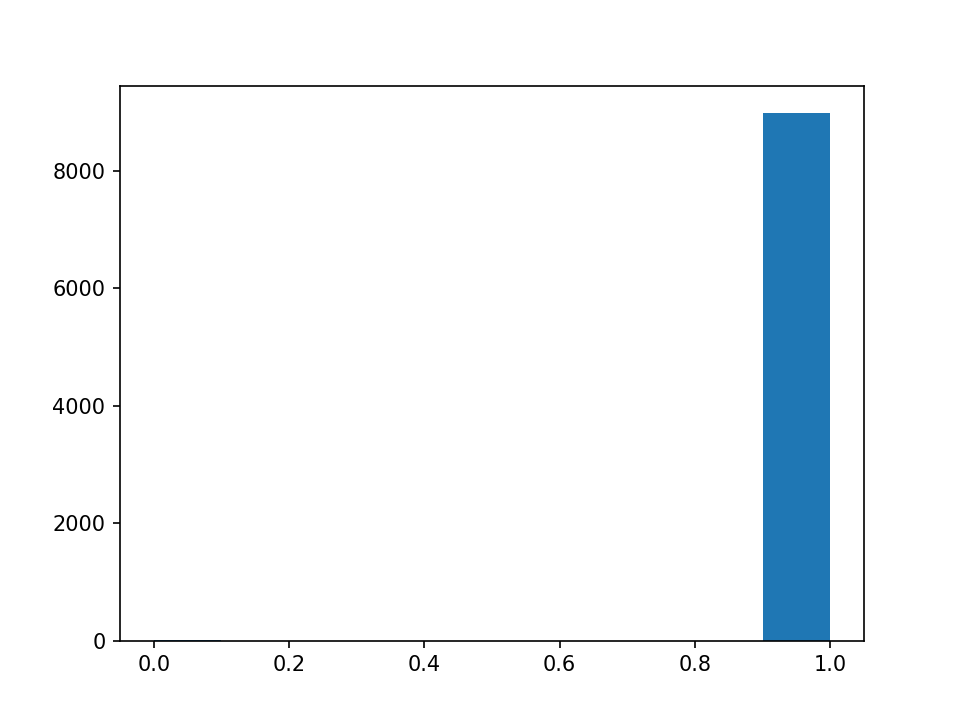
\includegraphics[scale=0.4]{p3histogram.png}
		\caption{Program 3 histogram }
	\end{figure}
	
		\subsubsection{Program 4}
		
		\begin{figure}[h]
			\centering
			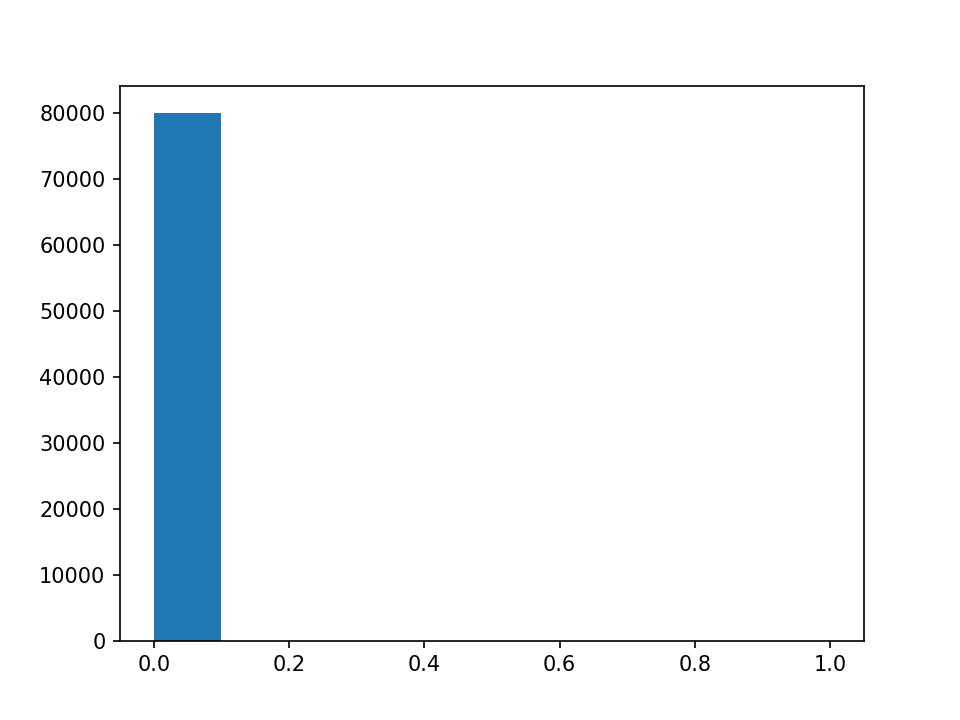
\includegraphics[scale=0.4]{p4histogram.png}
			\caption{Program 4 histogram }
		\end{figure}
	
%	\bibliography{research.bib}
%	\bibliographystyle{plain}
	
	
\end{document}